\subsection{UC 11 - Amministrazione - Gestione utenti}

		\begin{figure}[H]
			\centering
			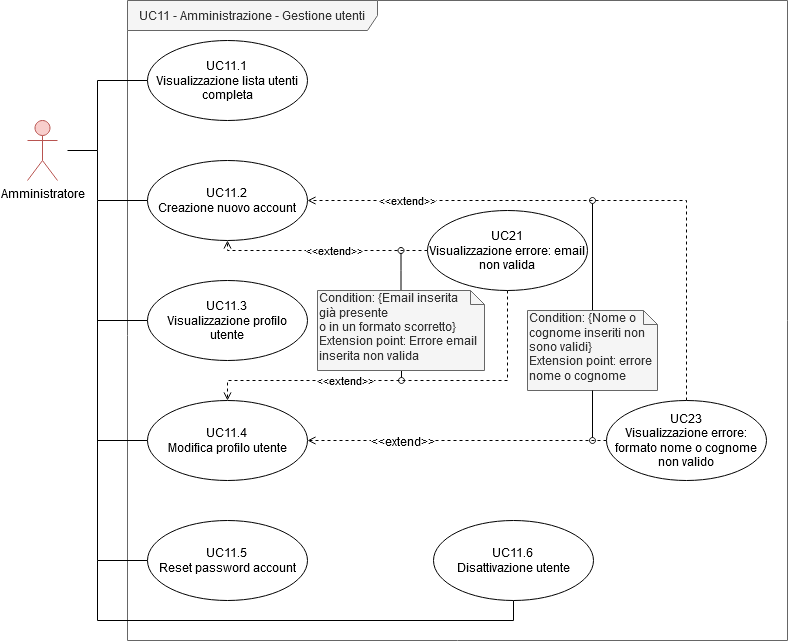
\includegraphics[scale=0.60]{res/images/uc11}
			\caption{Diagramma che descrive la gestione utenti a livello amministrativo.}
		\end{figure}

		\begin{itemize}
			\item \textbf{Attori Primari}: Amministratore.
			\item \textbf{Descrizione}: L'utente può navigare nell'area gestionale di tutti gli utenti del sistema. Può visualizzare e gestire questi utenti. 
			\item \textbf{Precondizione}: L'utente risulta autenticato nella web app e naviga nella gestione utenti per amministratori.
			\item \textbf{Postcondizione}: L'utente ha visualizzato o gestito gli utenti all'interno del sistema. 
			\item \textbf{Scenario Principale}:
			\begin{enumerate}
				\item{L'utente visualizza o gestisce gli utenti censiti dal sistema}
			\end{enumerate}	
		\end{itemize}

			\subsubsection{UC 11.1 - Visualizzazione lista utenti completa}
			\begin{itemize}
				\item \textbf{Attori Primari}: Amministratore.
				\item \textbf{Descrizione}: L'utente può visualizzare una lista con nome, cognome, mail ed ente di appartenenza di tutti gli utenti censiti nel sistema.
				\item \textbf{Precondizione}: L'utente naviga nella gestione utenti per amministratori.
				\item \textbf{Postcondizione}: L'utente visualizza la lista degli utenti registrati al sistema.
				\item \textbf{Scenario Principale}:
				\begin{enumerate}
					\item{L'utente visualizza la lista degli utenti registrati al sistema}
				\end{enumerate}	
			\end{itemize}
			
			\subsubsection{UC 11.2 - Creazione nuovo account}
			\begin{itemize}
				\item \textbf{Attori Primari}: Amministratore.
				\item \textbf{Descrizione}: L'utente può creare un nuovo account che viene inserito nel sistema e assegnato a un ente.
				\item \textbf{Precondizione}: L'utente naviga nella gestione utenti per amministratori.
				\item \textbf{Postcondizione}: L'utente ha creato un nuovo account.
				\item \textbf{Scenario Principale}:
				\begin{enumerate}
					\item{L'utente deve compilare dei campi con i dati dell'utente da aggiungere;}
					\item{L'utente compila il campo per la email;}
					\item{L'utente compila il campo per il nome;}
					\item{L'utente compila il campo per il cognome;}
					\item{L'utente seleziona l'ente a cui assegnare il nuovo account tra quelli disponibili;}
					\item{L'utente seleziona la tipologia di utente;}
					\item{L'utente ha aggiunto un nuovo utente al sistema.}
				\end{enumerate}	
				\item \textbf{Estensioni}:
				\begin{itemize}
					\item L'utente inserisce un email non valida (UC 21)
					\item L'utente inserisce un nome o cognome non validi (UC 23)
				\end{itemize}
			\end{itemize}
			
			\paragraph{UC 11.2.1 - Inserimento email}
			\begin{itemize}
				\item \textbf{Attori Primari}: Amministratore.
				\item \textbf{Descrizione}: L'utente sta creando un nuovo account che verrà inserito nel sistema e deve compilare un campo per la email. Il campo è obbligatorio.
				\item \textbf{Precondizione}: L'utente sta compilando i campi richiesti per l'aggiunta di un nuovo utente.
				\item \textbf{Postcondizione}: L'utente ha compilato il campo richiesto.
				\item \textbf{Scenario Principale}:
				\begin{enumerate}
					\item{L'utente compila il campo per la email;}
				\end{enumerate}	
			\end{itemize}

			\paragraph{UC 11.2.2 - Inserimento nome}
			\begin{itemize}
				\item \textbf{Attori Primari}: Amministratore.
				\item \textbf{Descrizione}: L'utente sta creando un nuovo account che verrà inserito nel sistema e deve compilare un campo per il nome. Il campo è obbligatorio.
				\item \textbf{Precondizione}: L'utente sta compilando i campi richiesti per l'aggiunta di un nuovo utente.
				\item \textbf{Postcondizione}: L'utente ha compilato il campo richiesto.
				\item \textbf{Scenario Principale}:
				\begin{enumerate}
					\item{L'utente compila il campo per il nome;}
				\end{enumerate}	
			\end{itemize}

			\paragraph{UC 11.2.3 - Inserimento cognome}
			\begin{itemize}
				\item \textbf{Attori Primari}: Amministratore.
				\item \textbf{Descrizione}: L'utente sta creando un nuovo account che verrà inserito nel sistema e deve compilare un campo per il cognome. Il campo è obbligatorio.
				\item \textbf{Precondizione}: L'utente sta compilando i campi richiesti per l'aggiunta di un nuovo utente.
				\item \textbf{Postcondizione}: L'utente ha compilato il campo richiesto.
				\item \textbf{Scenario Principale}:
				\begin{enumerate}
					\item{L'utente compila il campo per il cognome;}
				\end{enumerate}	
			\end{itemize}

			\paragraph{UC 11.2.4 - Selezione ente per il nuovo utente}
			\begin{itemize}
				\item \textbf{Attori Primari}: Amministratore.
				\item \textbf{Descrizione}: L'utente sta creando un nuovo account che verrà inserito nel sistema e deve compilare un campo che richiede a quale ente assegnare l'utente, tra quelli disponibili. Il campo è obbligatorio.
				\item \textbf{Precondizione}: L'utente sta compilando i campi richiesti per l'aggiunta di un nuovo utente.
				\item \textbf{Postcondizione}: L'utente ha compilato il campo richiesto.
				\item \textbf{Scenario Principale}:
				\begin{enumerate}
					\item{L'utente seleziona l'ente a cui assegnare il nuovo account tra quelli disponibili;}
				\end{enumerate}	
			\end{itemize}

			\paragraph{UC 11.2.5 - Selezione tipologia utente}
			\begin{itemize}
				\item \textbf{Attori Primari}: Amministratore.
				\item \textbf{Descrizione}: L'utente sta creando un nuovo account che verrà inserito nel sistema e deve compilare un campo che richiede a quale tipologia assegnare l'utente. Il campo è obbligatorio. Le tipologie disponibili sono:
				\begin{itemize}
					\item Membro;
					\item Moderatore ente.
				\end{itemize}
				\item \textbf{Precondizione}: L'utente sta compilando i campi richiesti per l'aggiunta di un nuovo utente.
				\item \textbf{Postcondizione}: L'utente ha compilato il campo richiesto.
				\item \textbf{Scenario Principale}:
				\begin{enumerate}
					\item{L'utente seleziona la tipologia di utente per il nuovo account;}
				\end{enumerate}	
			\end{itemize}

			\subsubsection{UC 11.3 - Visualizzazione profilo utente}
			\begin{itemize}
				\item \textbf{Attori Primari}: Amministratore.
				\item \textbf{Descrizione}: L'utente vuole visualizzare le informazioni del profilo di un utente presente nel sistema, quali: nome, cognome, username Telegram (se presente), opzione di autenticazione a due fattori (attiva o meno) ed ente di appartenenza.
				\item \textbf{Precondizione}: L'utente naviga all'interno della gestione utenti.
				\item \textbf{Postcondizione}: L'utente ha visualizzato le informazioni dell'utente selezionato.
				\item \textbf{Scenario Principale}:
				\begin{enumerate}
					\item{L'utente seleziona un utente dalla lista degli utenti;}
					\item{L'utente visualizza le informazioni dell'utente selezionato.}
				\end{enumerate}
			\end{itemize}


			\subsubsection{UC 11.4 - Modifica profilo utente}
			\begin{itemize}
				\item \textbf{Attori Primari}: Amministratore.
				\item \textbf{Descrizione}: L'utente modifica il profilo dell'utente selezionato dalla lista degli utenti.
				\item \textbf{Precondizione}: L'utente naviga all'interno della gestione utenti.
				\item \textbf{Postcondizione}: L'utente ha modificato l'utente selezionato.
				\item \textbf{Scenario Principale}:
				\begin{enumerate}
					\item L'utente seleziona un account utente che vuole modificare;
					\item L'utente deve compilare alcuni campi per proseguire nella modifica dell'utente selezionato;
					\item{L'utente modifica il campo per la email (UC 11.4.1);}
					\item{L'utente modifica il campo per il nome (UC 11.4.2);}
					\item{L'utente modifica il campo per il cognome (UC 11.4.3);}
					\item{L'utente modifica il campo Username \glock{Telegram} (UC 11.4.4);}
					\item{L'utente seleziona l'ente a cui assegnare il nuovo account tra quelli disponibili (UC 11.4.5);}
					\item{L'utente seleziona la tipologia di utente (UC 11.4.6);}
					\item{L'utente seleziona la preferenza per l'autenticazione a due fattori di quell'account (UC 11.4.7);}
					\item{L'utente ha compilato tutti i campi e conferma.}
				\end{enumerate}	
				\item \textbf{Estensioni}:
				\begin{itemize}
					\item L'utente inserisce una email non valida (UC 21);
					\item L'utente inserisce un nome o cognome non validi (UC 23).
				\end{itemize}
			\end{itemize}
			
				\paragraph{UC 11.4.1 - Modifica email}
				\begin{itemize}
					\item \textbf{Attori Primari}: Amministratore.
					\item \textbf{Descrizione}: L'utente sta modificando un account esistente censito a sistema e deve compilare un campo per la email. Il campo è obbligatorio.
					\item \textbf{Precondizione}: L'utente sta compilando i campi richiesti per la modifica di un utente.
					\item \textbf{Postcondizione}: L'utente ha compilato il campo richiesto.
					\item \textbf{Scenario Principale}:
					\begin{enumerate}
						\item{L'utente compila il campo per la email.}
					\end{enumerate}	
				\end{itemize}

				\paragraph{UC 11.4.2 - Modifica nome}
				\begin{itemize}
					\item \textbf{Attori Primari}: Amministratore.
					\item \textbf{Descrizione}: L'utente sta modificando un account esistente censito a sistema e deve compilare un campo per il nome. Il campo è obbligatorio.
					\item \textbf{Precondizione}: L'utente sta compilando i campi richiesti per la modifica di un utente.
					\item \textbf{Postcondizione}: L'utente ha compilato il campo richiesto.
					\item \textbf{Scenario Principale}:
					\begin{enumerate}
						\item{L'utente compila il campo per il nome.}
					\end{enumerate}	
				\end{itemize}

				\paragraph{UC 11.4.3 - Modifica cognome}
				\begin{itemize}
					\item \textbf{Attori Primari}: Amministratore.
					\item \textbf{Descrizione}: L'utente sta modificando un account esistente censito a sistema e deve compilare un campo per il cognome. Il campo è obbligatorio.
					\item \textbf{Precondizione}: L'utente sta compilando i campi richiesti per la modifica di un utente.
					\item \textbf{Postcondizione}: L'utente ha compilato il campo richiesto.
					\item \textbf{Scenario Principale}:
					\begin{enumerate}
						\item{L'utente compila il campo per il cognome.}
					\end{enumerate}	
				\end{itemize}

				\paragraph{UC 11.4.4 - Modifica username Telegram}
				\begin{itemize}
					\item \textbf{Attori Primari}: Amministratore.
					\item \textbf{Descrizione}: L'utente sta modificando un account esistente censito a sistema e deve compilare un campo per lo username \glock{Telegram}. Il campo è obbligatorio.
					\item \textbf{Precondizione}: L'utente sta compilando i campi richiesti per la modifica di un utente.
					\item \textbf{Postcondizione}: L'utente ha compilato il campo richiesto.
					\item \textbf{Scenario Principale}:
					\begin{enumerate}
						\item{L'utente compila il campo per lo username \glock{Telegram}.}
					\end{enumerate}	
				\end{itemize}

				\paragraph{UC 11.4.5 - Modifica ente di appartenenza}
				\begin{itemize}
					\item \textbf{Attori Primari}: Amministratore.
					\item \textbf{Descrizione}: L'utente sta modificando un account esistente censito a sistema e deve compilare un campo per assegnare quell'utente a uno degli enti censiti da sistema. Il campo è obbligatorio.
					\item \textbf{Precondizione}: L'utente sta compilando i campi richiesti per la modifica di un utente.
					\item \textbf{Postcondizione}: L'utente ha compilato il campo richiesto.
					\item \textbf{Scenario Principale}:
					\begin{enumerate}
						\item{L'utente seleziona l'ente a cui assegnare il nuovo account tra quelli disponibili.}
					\end{enumerate}	
				\end{itemize}

				\paragraph{UC 11.4.6 - Modifica tipologia di utente}
				\begin{itemize}
					\item \textbf{Attori Primari}: Amministratore.
					\item \textbf{Descrizione}: L'utente sta modificando un account esistente censito a sistema e deve compilare un campo per assegnare la tipologia di account per un dato utente. Il campo è obbligatorio. Le tipologie disponibili sono:
					\begin{itemize}
						\item Membro;
						\item Moderatore ente.
					\end{itemize}
					\item \textbf{Precondizione}: L'utente sta compilando i campi richiesti per la modifica di un utente.
					\item \textbf{Postcondizione}: L'utente ha compilato il campo richiesto.
					\item \textbf{Scenario Principale}:
					\begin{enumerate}
						\item{L'utente seleziona la tipologia di account da assegnare per un utente in base a quelli disponibili.}
					\end{enumerate}	
				\end{itemize}

				\paragraph{UC 11.4.7 - Modifica preferenza per l'autenticazione a due fattori}
				\begin{itemize}
					\item \textbf{Attori Primari}: Amministratore.
					\item \textbf{Descrizione}: L'utente sta modificando un account esistente censito a sistema e deve compilare un campo per la preferenza di attivazione dell'autenticazione a due fattori con \glock{Telegram}. Il campo è obbligatorio. Le preferenze disponibili sono:
					\begin{itemize}
						\item Abilitata;
						\item Disabilitata.
					\end{itemize}
					\item \textbf{Precondizione}: L'utente sta compilando i campi richiesti per la modifica di un utente.
					\item \textbf{Postcondizione}: L'utente ha compilato il campo richiesto.
					\item \textbf{Scenario Principale}:
					\begin{enumerate}
						\item{L'utente seleziona la preferenza per l'autenticazione a due fattori.}
					\end{enumerate}	
				\end{itemize}



			\subsubsection{UC 11.5 - Reset password account}
			\begin{itemize}
				\item \textbf{Attori Primari}: Amministratore.
				\item \textbf{Descrizione}: L'utente vuole resettare la password di un account utente censito nel sistema.
				\item \textbf{Precondizione}: L'utente naviga all'interno della gestione utenti per l'amministrazione.
				\item \textbf{Postcondizione}: L'utente ha resettato la password dell'account selezionato.
				\item \textbf{Scenario Principale}:
				\begin{enumerate}
					\item{L'utente seleziona un utente diverso tra quelli disponibili cui vuole resettare la password;}
					\item{L'utente ha resettato la password all'utente di sistema.}
				\end{enumerate}		
			\end{itemize}

			
			\subsubsection{UC 11.6 - Disattivazione utente}
			\begin{itemize}
				\item \textbf{Attori Primari}: Amministratore.
				\item \textbf{Descrizione}: L'utente vuole disattivare l'account di un utente attualmente attivo.
				\item \textbf{Precondizione}: L'utente naviga all'interno della gestione utenti per l'amministrazione.
				\item \textbf{Postcondizione}: L'utente ha disattivato l'account dell'utente selezionato.
				\item \textbf{Scenario Principale}:
				\begin{enumerate}
					\item{L'utente seleziona un utente tra quelli disponibili da disattivare;}
					\item{L'utente ha disattivato l'utente dal sistema.}
				\end{enumerate}		
			\end{itemize}

			
			